% Created 2017-03-01 Wed 20:38
\documentclass[10pt]{article}
\usepackage[utf8]{inputenc}
\usepackage[T1]{fontenc}
\usepackage{fixltx2e}
\usepackage{graphicx}
\usepackage{longtable}
\usepackage{float}
\usepackage{wrapfig}
\usepackage{rotating}
\usepackage[normalem]{ulem}
\usepackage{amsmath}
\usepackage{textcomp}
\usepackage{marvosym}
\usepackage{wasysym}
\usepackage{amssymb}
\tolerance=1000
\usepackage{natbib}
\usepackage[linktocpage,pdfstartview=FitH,colorlinks,
linkcolor=blue,anchorcolor=blue,
citecolor=blue,filecolor=blue,menucolor=blue,urlcolor=blue]{hyperref}
\usepackage[margin=2cm]{geometry}
\pagenumbering{gobble}
\usepackage{wrapfig}
\usepackage{multicol}
\setlength\columnsep{20pt}
\author{Alejandro Rodríguez Salamanca - r0650814@student.kuleuven.be - Erasmus}
\date{}
\title{Artificial Neural Networks: Session 4}
\begin{document}

\maketitle
\begin{multicols}{2}

 
  
  \section*{Digit Classification with Stacked Autoencoders}
  The aim of this exercise is to classify digits using a deep neural network. The problem
  with this type of networks is that it becomes difficult to train them, as they have
  several layers, each one learning a different abstraction of the features. To solve this
  problem, one layer is trained at a time, in an unsupervised way, using autoencoders. Finally,
  the last layer is trained using the \texttt{softmax} activation function in a supervised way,
  and then all the layers are joined together.

  Training and executing a network with two hidden layers in the dataset of digital numbers we get
  an accuracy of 81.9\%. This result can be improved retraining the network one more time in
  a supervised fashion using backpropagation. This technique is also known as fine tuning.
  The confusion matrix shows in this case an accuracy of 99.7\%.

  If it is executed in a normal neural network with one hidden layer, the accurary is 97\%,
  and with two hidden layers, 95.84\%.

  Adding one more layer to the deep neural network causes a decrease in the accuracy to values
  around 20\%. This phenomena can be caused by an extra complexity that induces overfitting.
  After the fine tuning process, the accuracy increases to 97\%, still lower than the one
  obtained with two layers.

  

  \section*{Convolutional Neural Networks: questions}
  A convolutional neural network (CNN, or ConvNet) is a type of feed-forward artificial
  neural network in which the connectivity pattern between its neurons is inspired by
  the organization of the animal visual cortex. They have wide applications in image and
  video recognition, recommender systems and natural language processing.
  In this exercise we are going to see how we can apply a CNN to image recognition.

  A simple CNN could have the following architecture: INPUT - CONV - RELU - POOL - FC.

  \begin{center}
    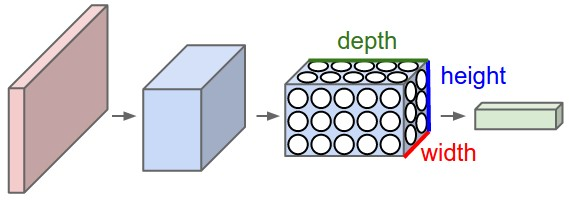
\includegraphics[width=\linewidth]{img/cnn}
  \end{center}

  \begin{itemize}
  \item INPUT: will hold the raw pixel values of the image,
    in this case an image of width 227, height 227, and with three color channels R,G,B.
    
  \item CONV layer will compute the output of neurons that are connected to local regions
    in the input, each computing a dot product between their weights and a small region
    they are connected to in the input volume. This may result in volume such as
    [227x227x96] if we decided to use 96 filters.

  \item RELU layer will apply an elementwise activation function,
    such as the $max(0,x)$ thresholding at zero.
    This leaves the size of the volume unchanged

  \item POOL layer will perform a downsampling operation along the spatial
    dimensions (width, height).

  \item FC (i.e. fully-connected) layer will compute the class scores.
    
  \end{itemize}
 
  
     \begin{center}
	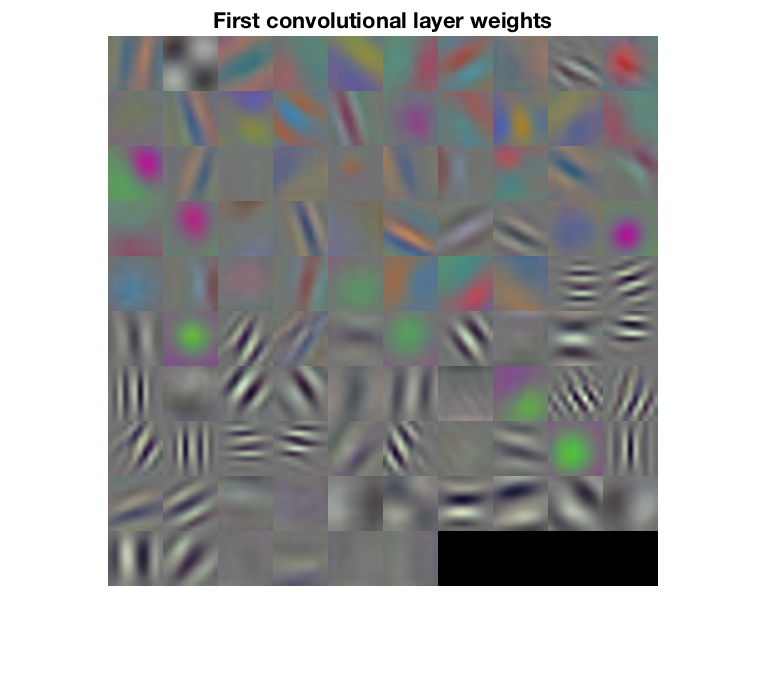
\includegraphics[width=\linewidth]{img/layerweights}
      \end{center}

      In layers 1 to 5 we can find the input layer, a convolution layer, a ReLU layer,
      a Cross Channel Normalization layer and a Max Pooling layer. Knowing that
      a ReLU and a Cross Channel Normalization layer do not affect the dimension of the input,
      the dimension of the input at layer 6 would be  $27 \times 27 \times 96$.
      
      First, the image of $227 \times 227 \times 3$ is convolved with $11 \times 11 \times 3$
      filters at stride 4, using 96 filters,
      which gives an output of $55 \times 55 \times 96$. ($(227-11)/4+1 = 55$).
      Then, a ReLU and a Cross Channel normalization layer are applied. As we already know,
      this two layers do not affect the dimension of the input, so we reach the Max Pooling layer.

      A Max Pooling layer accepts a volume of size $W_{1} \times H_{1} \times D_{1}$ and requires two
      parameters, their spatial extent $F$ and the stride $S$.
      It produces a volume of size $W_{2} x H_{2} x D_{2}$ where:
      \begin{itemize}
        \item $W_{2} = (W_{1} - F) / S + 1$
        \item $H_{2} = (H_{1} - F) / S + 1$
        \item $D_{2} = D_{1}$
     \end{itemize}

     \begin{center}
       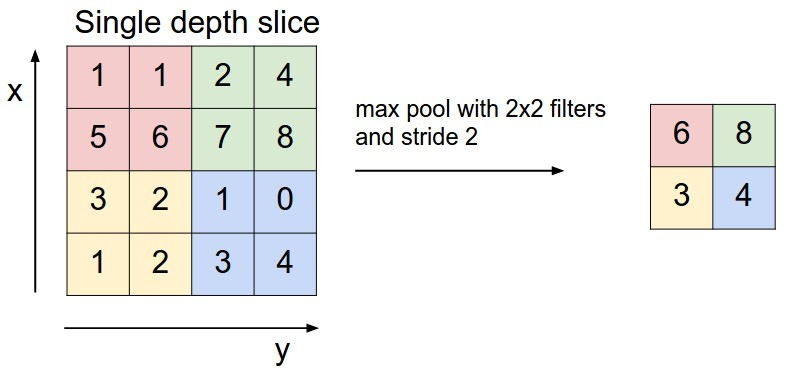
\includegraphics[width=\linewidth]{img/maxpool}
     \end{center}

      In our case, size of the output after this layer would be $27 \times 27 \times 96$.
     

    The number of neurons used for the final classification task is 1000. It can be seen
    in both the network architecture, in which the last layer is \texttt{'classificationLayer'
      Classification Output         cross-entropy with 'n01440764', 'n01443537', and 998 other classes}
    and when executing \texttt{numel(convnet.Layers(end).ClassNames)}, which returns 1000.
    But this model was trained to solve a 1000-way classification problem. To solve our
    problem, it should be adapted to have three neurons in the classification layer, one for each
    one of the possible classes, airplanes, ferry, and laptop.

\end{multicols}
\end{document}
